\documentclass[a4paper,class=article,border=5pt,tikz]{standalone}
\usetikzlibrary{shapes.geometric}

\tikzset{
  box/.style={
    regular polygon,
    regular polygon sides=6,
    minimum size=10mm,
    inner sep=0mm,
    outer sep=0mm,
    rotate=0,
  draw
  }
}

\begin{document}

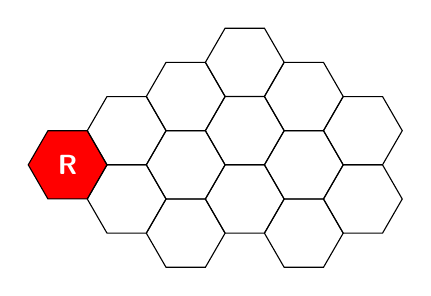
\begin{tikzpicture}[x=7.5mm,y=4.34mm]
    \node[box,fill=red,text=white] at (1,1) {\textbf{\textsf{R}}};
    \node[box] at (2,2) {};
    \node[box] at (3,3) {};
    \node[box] at (4,4) {};
    \node[box] at (2,0) {};
    \node[box] at (3,1) {};
    \node[box] at (4,2) {};
    \node[box] at (5,3) {};
    \node[box] at (3,-1) {};
    \node[box] at (4,0) {};
    \node[box] at (5,1) {};
    \node[box] at (6,2) {};
    \node[box] at (5,-1) {};
    \node[box] at (6,0) {};
\end{tikzpicture}


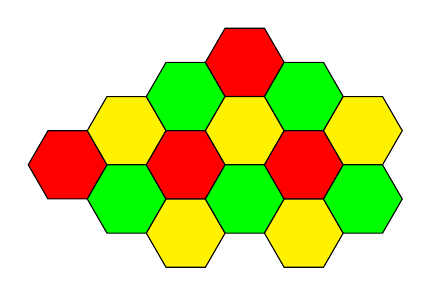
\begin{tikzpicture}[x=7.5mm,y=4.34mm]
    \node[box,fill=red] at (1,1) {};
    \node[box,fill=yellow] at (2,2) {};
    \node[box,fill=green] at (3,3) {};
    \node[box,fill=red] at (4,4) {};
    \node[box,fill=green] at (2,0) {};
    \node[box,fill=red] at (3,1) {};
    \node[box,fill=yellow] at (4,2) {};
    \node[box,fill=green] at (5,3) {};
    \node[box,fill=yellow] at (3,-1) {};
    \node[box,fill=green] at (4,0) {};
    \node[box,fill=red] at (5,1) {};
    \node[box,fill=yellow] at (6,2) {};
    \node[box,fill=yellow] at (5,-1) {};
    \node[box,fill=green] at (6,0) {};
\end{tikzpicture}



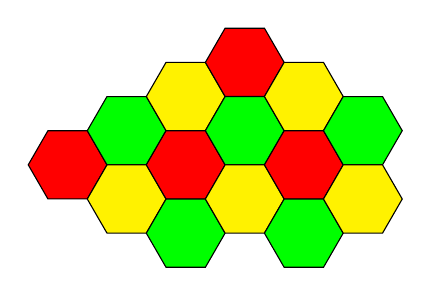
\begin{tikzpicture}[x=7.5mm,y=4.34mm]
    \node[box,fill=red] at (1,1) {};
    \node[box,fill=green] at (2,2) {};
    \node[box,fill=yellow] at (3,3) {};
    \node[box,fill=red] at (4,4) {};
    \node[box,fill=yellow] at (2,0) {};
    \node[box,fill=red] at (3,1) {};
    \node[box,fill=green] at (4,2) {};
    \node[box,fill=yellow] at (5,3) {};
    \node[box,fill=green] at (3,-1) {};
    \node[box,fill=yellow] at (4,0) {};
    \node[box,fill=red] at (5,1) {};
    \node[box,fill=green] at (6,2) {};
    \node[box,fill=green] at (5,-1) {};
    \node[box,fill=yellow] at (6,0) {};
\end{tikzpicture}
\end{document}
